\subsection{Exklusiv-Oder-Gatter (XOR) aufgebaut aus NAND-Gattern} % (fold)
\label{sub:Exklusiv-Oder-Gatter (XOR) aufgebaut aus NAND-Gattern}
\begin{frame}
    \frametitle{XOR aus NAND-Gattern}
    \framesubtitle{}
     \begin{columns}[c]
         \column{0.5\textwidth}
            \begin{itemize}
                \item NAND Schaltung:
                    \boxed{
                        \begin{tabular}{c|c||c}
                            A & B & Y \\
                            \hline
                            1 & 0 & 1 \\
                            0 & 1 & 1 \\
                            0 & 0 & 1 \\
                            1 & 1 & 0
                        \end{tabular}
                        }
                \item XOR Schaltung:
                    \boxed{
                        \begin{tabular}{c|c||c}
                            A & B & Y \\
                            \hline
                            1 & 0 & 1 \\
                            0 & 1 & 1 \\
                            0 & 0 & 0 \\
                            1 & 1 & 0
                        \end{tabular}
                        }
            \end{itemize}
         \column{0.5\textwidth}
            \begin{figure}[H]
            \begin{center}
                    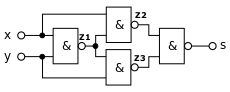
\includegraphics[scale=0.7]{./img/schaltung/XOR_NAND.png}
            \end{center}
            \end{figure}
     \end{columns}
\end{frame}

\begin{frame}
    \frametitle{Funktionsweise}
    \framesubtitle{}
    \begin{columns}[c]
        \column{0.4\textwidth}
            \begin{center}
                \boxed{
                    \begin{tabular}{c|c||c|c|c||c}
                    A & B & Z1 & Z2 & Z3 & S \\
                    \hline
                    1 & 0 & 1 & 0 & 1 & 1
                    \end{tabular}
                }
            \end{center}
        \column{0.6\textwidth}
            \begin{figure}[H]
            \begin{center}
                    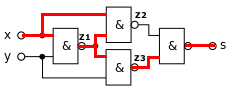
\includegraphics[scale=0.7]{./img/schaltung/xornand_fun_10.png}
            \end{center}
            \end{figure}
    \end{columns}
\end{frame}

\begin{frame}
    \frametitle{Funktionsweise}
    \framesubtitle{}
    \begin{columns}[c]
        \column{0.4\textwidth}
            \begin{center}
                \boxed{
                    \begin{tabular}{c|c||c|c|c||c}
                    A & B & Z1 & Z2 & Z3 & S \\
                    \hline
                    1 & 0 & 1 & 0 & 1 & 1 \\
                    0 & 1 & 1 & 1 & 0 & 1 
                    \end{tabular}
                }
            \end{center}
        \column{0.6\textwidth}
            \begin{figure}[H]
            \begin{center}
                    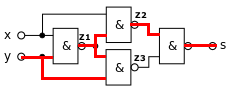
\includegraphics[scale=0.7]{./img/schaltung/xornand_fun_01.png}
            \end{center}
            \end{figure}
    \end{columns}
\end{frame}

\begin{frame}
    \frametitle{Funktionsweise}
    \framesubtitle{}
    \begin{columns}[c]
        \column{0.4\textwidth}
            \begin{center}
                \boxed{
                    \begin{tabular}{c|c||c|c|c||c}
                    A & B & Z1 & Z2 & Z3 & S \\
                    \hline
                    1 & 0 & 1 & 0 & 1 & 1 \\
                    0 & 1 & 1 & 1 & 0 & 1 \\
                    0 & 0 & 1 & 1 & 1 & 0 
                    \end{tabular}
                }
            \end{center}
        \column{0.6\textwidth}
            \begin{figure}[H]
            \begin{center}
                    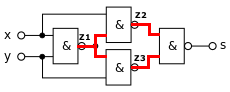
\includegraphics[scale=0.7]{./img/schaltung/xornand_fun_00.png}
            \end{center}
            \end{figure}
    \end{columns}
\end{frame}
\begin{frame}
    \frametitle{Funktionsweise}
    \framesubtitle{}
    \begin{columns}[c]
        \column{0.4\textwidth}
            \begin{center}
                \boxed{
                    \begin{tabular}{c|c||c|c|c||c}
                    A & B & Z1 & Z2 & Z3 & S \\
                    \hline
                    1 & 0 & 1 & 0 & 1 & 1 \\
                    0 & 1 & 1 & 1 & 0 & 1 \\
                    0 & 0 & 1 & 1 & 1 & 0 \\
                    1 & 1 & 0 & 1 & 1 & 0 
                    \end{tabular}
                }
            \end{center}
        \column{0.6\textwidth}
            \begin{figure}[H]
            \begin{center}
                    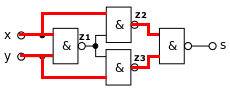
\includegraphics[scale=0.7]{./img/schaltung/xornand_fun_11.png}
            \end{center}
            \end{figure}
    \end{columns}
    \pause
    \begin{block}{}
        \begin{center}
        $\rightarrow$ XOR-Schaltung
        \end{center}
    \end{block}
\end{frame}
% subsection Exklusiv-Oder-Gatter (XOR) aufgebaut aus NAND-Gattern (end)
